\chapter{Measurement of the realized circuit in the time domain}
\label{ch:measurement}
% The heart of the thesis, comprising a presentation of the functioning system and thus the culmination of the work. Important is an analysis of the results as well as a comparison with the state of the art. The reader should understand in this section why you should be awarded a MSc degree.

%The aim of the measurement was to show the feasibility to generate (different) signals, using the two bit resolution of the circuit.

The aim of the measurement was to show the generation of different signals.\\
With respect to produce a decent signal waveform at the output, the assembled hybrid test circuit was terminated with a \SI{50}{\ohm} termination and a \SI{3.3}{\nano\farad} capacitance, respectively.
In contrast to the calculated capacitance of \SI{20}{\pico \farad} in chapter \ref{ch:design}, a over dimensioned capacitor of \SI{3.3}{\nano\farad} terminated the output to ensure that the signal would not be clipped.
%The assembled hybrid test circuit was measured with respect to produce a decent signal waveform at its output in the time domain.
%For the measurement (in the time domain) the output of the realized circuit was terminated with a \SI{50}{\ohm} termination and a \SI{3.3}{\nano\farad} capacitance, respectively.
%The output voltage waveform was measured with a \SI{50}{\ohm} termination and a \SI{3.3}{\nano\farad} capacitance, respectively.
%A discrete passive capacitor replaced the calculated impedance in chapter \ref{ch:design} used for the simulation.

After the calibration of the measurement instruments a stability check was performed to ensure that the test circuit do not oscillate.
%Otherwise the circuit (would oscillate and) could damage the chips.
In a next step the output of the circuit was measured with a resistive load to show the function of the push-pull stage.
%For the input control voltage a \gls{ab:awg} from Keysight Technologies was used.
The correct functioning of the push-pull stage enabled the measurement with a capacitive load to synthesize a triangular waveform.
In order to avoid any kind of damage the measurement was performed with low \gls{ab:dc} supply voltages.


\section{Measurement setup}
An overview of the measurement setup is given in Figure \ref{fig:SchematicMeasSetup}.\\
%To ensure the instruments to work properly without taking damage their specifications have to be complied.
%In order to get good measurement results some requirements have to be fulfilled.
%an overview of the measurement setup is given.
%In order to comply specification of the measurement instruments and avoid them to be damaged, it was necessary to fulfil some conditions.
A signal generator generated a square wave signal with an amplitude of \SI{0.7}{\volt} and \SI{0.45}{\volt}, respectively.
As a square wave signal consists of several harmonics, the pre amplifier had to support a wide bandwidth.\\
The square wave of $Ch1$ \& $\overline{Ch1}$ and $Ch2$ \& $\overline{Ch2}$ of the \gls{ab:awg} is amplified by broadband amplifier G1 and G2, respectively.\\
A \gls{ab:dc} bias voltage is applied to the inputs of the \gls{ab:dut} to generate a square wave signal from $V_{low}$ = \SI{-10}{\volt} to $V_{high}$ = \SI{-5}{\volt}.
The voltage swing of \SI{5}{\volt} as well as the \gls{ab:dc} bias voltage were needed to ensure that the input transistors switch completely on and off.
%In order to ensure that the \gls{ab:hemt} base transistor at the input of the circuit is fully switched on and off a peak to peak value of \SI{5}{\volt} is needed.
%\SI{5}{\volt} peak to peak input signal is needed to ensure that the \gls{ab:hemt} is fully opened or fully closed.\\
Several power supplies provided the necessary \gls{ab:dc} supply voltages for the broadband amplifiers, bias tees and \gls{ab:dut}.\\
For the measurement of the push-pull stage an attenuator with \SI{20}{\decibel} attenuation was connected between the output of the \gls{ab:dut} and the input of the oscilloscope.
This attenuator ensured that the specifications of the oscilloscope (scope 1) were complied.\\
The measurement of the voltage across the load capacitance was done by another oscilloscope (scope 2) which provides a handy probe.
This probe allowed to measure the voltage directly on the output line of the hybrid test circuit.


\begin{figure}[htb!]
	\centering
  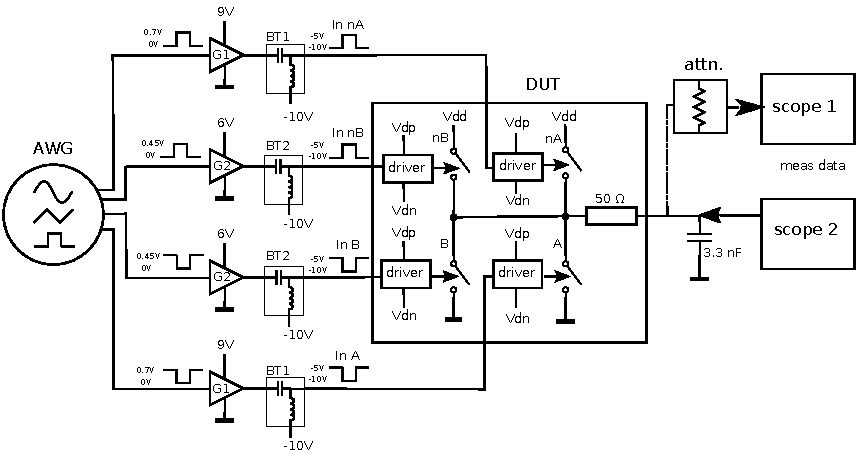
\includegraphics{meassetupschem.pdf}
	\caption{Schematic of time domain measurement setup}
	\label{fig:SchematicMeasSetup}
\end{figure}

%This signal is amplified by a pre power amplifier to get a decent voltage swing of \SI{5}{\volt}.
%This swing is needed to be sure to turn the \gls{ab:gan} \gls{ab:hemt} at the input of the circuit on and off.
%In addition to the swing another requirement is a \gls{ab:dc} offset of \SI{-10}{\volt}, because the transistor is a normally on device.
%The \gls{ab:dc} bias is fed through a bias tee to ensure that the output of the \gls{ab:awg} is not loaded.\\
%In fact that maximum input signal of the oscilloscope is at \SI{2}{\volt}, the signal provided by the circuit has to be attenuated.


The elements of the measurement setup were:
\begin{itemize}
	\item Signal generator: Keysight M8195A AWG
	\begin{itemize}
		\item $Ch1$ \& $\overline{Ch1}$: $V_{p-p}$ = \SI{0.7}{\volt} (square wave)
		\item $Ch2$ \& $\overline{Ch2}$: $V_{p-p}$ = \SI{0.45}{\volt} (square wave)
	\end{itemize}
	\item Broadband Amplifier
	\begin{itemize}
		\item G1: SHF803\\ gain = 17 dB (typ.), B = \SI{35}{\kilo \hertz} -  \SI{40}{\giga \hertz}
		\item G2: SHF804TL\\ gain = 21 dB (typ.), B = \SI{200}{\kilo \hertz} -  \SI{55}{\giga \hertz}
	\end{itemize}
	\item Bias Tee 
	\begin{itemize}
		\item BT1: SHF121A\\ B = \SI{50}{\kilo \hertz} -  \SI{65}{\giga \hertz}
		\item BT2: SHF121D\\ B = \SI{50}{\kilo \hertz} -  \SI{65}{\giga \hertz}
	\end{itemize}
	\item \gls{ab:dut}
	\item Power supplies
	\item Attenuator: 18B50W\\ B = \gls{ab:dc} -  \SI{18}{\giga \hertz}, Attenuation = 20 dB
	\item Capacitive load\\
	ceramic \gls{ab:smd} capacitor (\SI{3.3}{\nano \farad})
	\item Oscilloscope
	\begin{itemize}
		\item scope 1: DCA-X 86100D + 86118A (module)
		\item scope 2: DSO-X 3034A + HP 10432A (probe)
	\end{itemize}		
\end{itemize}

\begin{figure}[htb!]
	\centering
  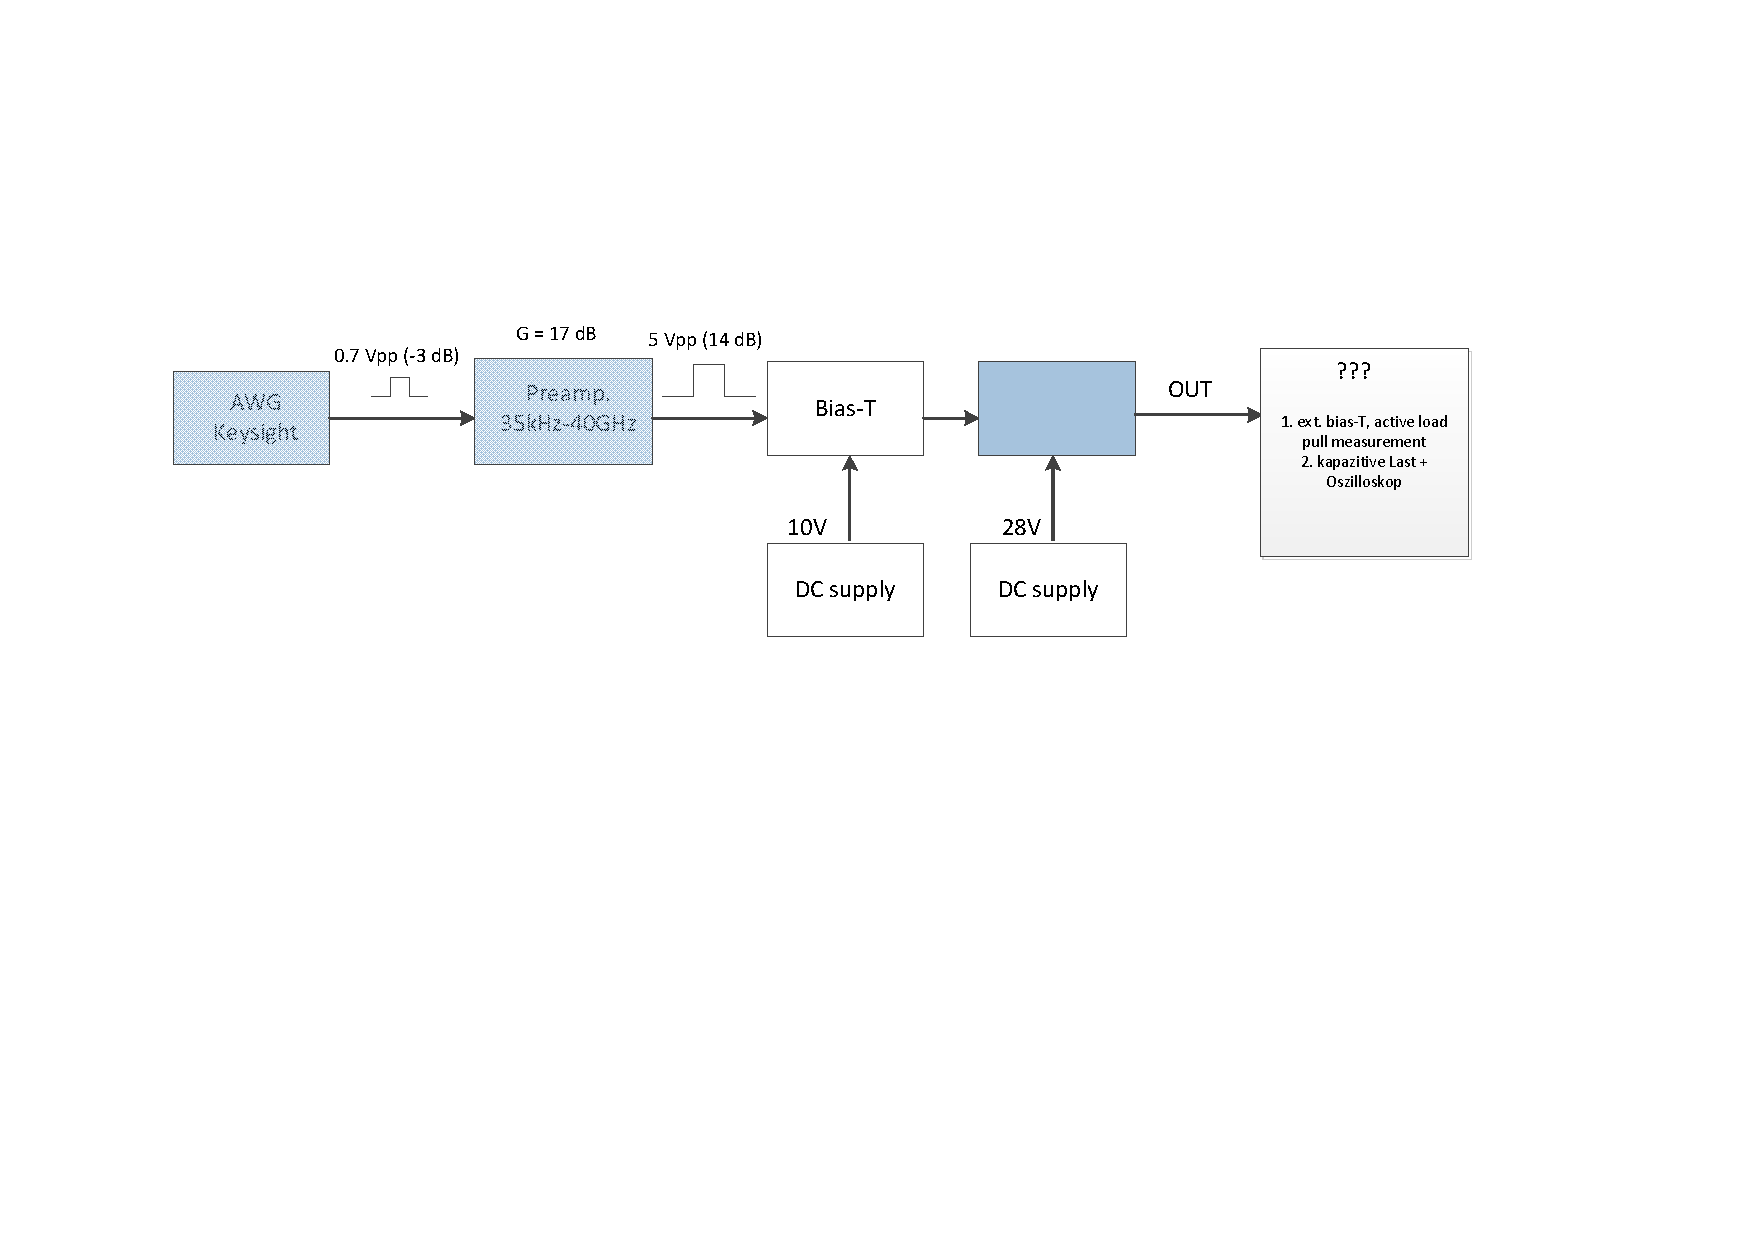
\includegraphics{MeasSetup.pdf}
	\caption{Photograph of measurement setup}
	\label{fig:PhotoMeasSetup}
\end{figure}

\section{Calibration and stability check}
Before performing the first measurement the instruments and used devices had to be calibrated.
The \gls{ab:awg} output amplitude had to be adjusted to the proper value depending on which pre amplifier is used, as the broadband amplifier differ in their gain.
The actual broadband amplifiers gain has to be checked as well as the proper configuration of the bias voltages.
These prerequisites are necessary to ensure a proper measurement.
After the calibration the first measurement checked the stability of the circuit.
Therefore the \gls{ab:dut} was supplied by its bias voltages and the current was checked if it stays constant.
Due to the fact that the current was stabilized after the transient time, it showed that the circuit is stable.
For this measurement the in- and output connectors were terminated with \SI{50}{\ohm} terminations.


\section{Time domain measurement of push-pull stage}
After checking stability of the \gls{ab:dut} a small signal is fed to its input.
Feeding a square wave signal (digital signal) to the input of the device its output switches between \gls{sy:Vdd} and GND potential.
This is done with the push-pull stage realized with multi chip assembling on a hybrid board.
%Having demonstrated the stability of the circuit, the next step was to show the function of the push-pull stage.
\textit{The hybrid board consists of four inputs which two are working in differential mode.}\\
Switching the output to \gls{sy:Vdd} needed an in phase control signal.
Two high side transistors should switch and fed the upper power rail which is \gls{sy:Vdd} to the output.
Meaning both power transistors have to switch at the same time to provide \gls{sy:Vdd} to the output.
While highside and lowside transistor both switched on the output is floating between \gls{sy:Vdd} and GND.\\
Figure \ref{fig:inputMeas} shows the square wave input control signal.
%This signal is generated using a \gls{ab:awg}.
%This \gls{ab:awg} is linear in amplification over a frequency range of \textit{???}.
The square wave signal form represents a digital signal with a data rate of 200Mbps while the fundamental analog frequency is at \SI{100}{\mega \hertz}.
The required peak to peak voltage is configured to be \SI{0.7}{\volt}.
The light grey signal represents one input stream while the darker grey signal represents the inverse one.
This signal represents a digital bit stream which is needed to control the circuit.
The data rate of the presented signal is 200 Mbps while the analog fundamental frequency is \SI{100}{\mega\hertz}.

\begin{figure}[htb!]
	\centering
  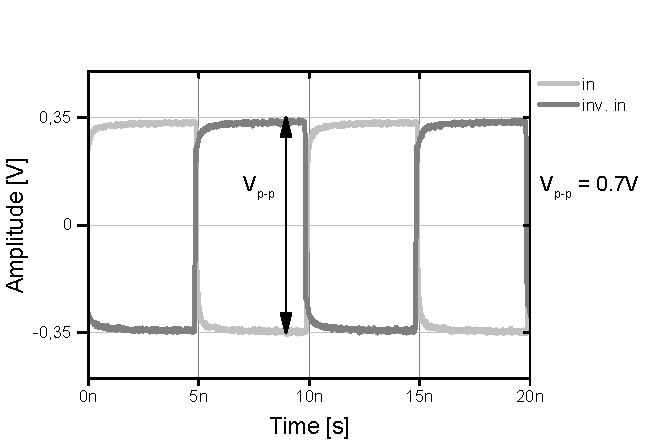
\includegraphics{inputVoltage.pdf}
	\caption{time domain measurement input control voltage}
	\label{fig:inputMeas}
\end{figure}


Using this input signal the circuit under test, with a \SI{50}{\ohm} termination, provides the output shown in figure \ref{fig:measRload100M}.

% signal to noise, signal  to quantisation noise ratio!

\begin{figure}[htb!]
	\centering
  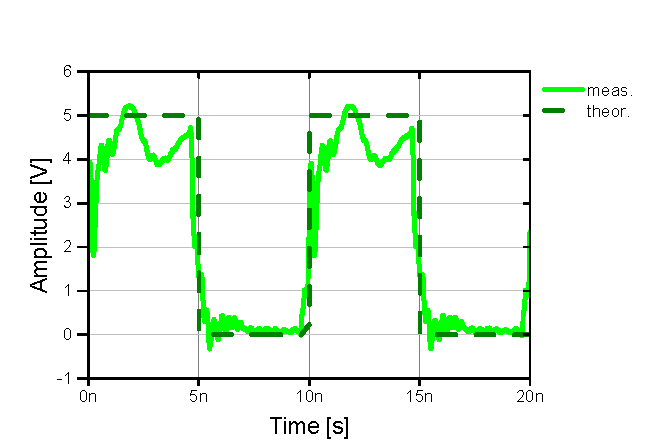
\includegraphics{100M_Rload_regression.pdf}
	\caption{Time domain measurement of output voltage with 50 Ohm termination}
	\label{fig:measRload100M}
\end{figure}

The light green signal is the measured data while the dashed line describes the ideal behaviour.
In an ideal world there would be neither rising nor falling time and the signal would switch between logical one and zero.\\
This figure demonstrate the proper functioning of the presented output push-pull stage, as the signal switches between Vdd and GND.
In addition to this it is demonstrated that the switches are very fast since the rising and falling edges are very steep.
The frequency accords with the input signal shown in figure \ref{fig:inputMeas}.

% RC-element with 50 Ohm transmission line. Charge time reduce due to the occurence of the 50 Ohm environment. tau = R*C = 63% Vmax

\section{Time domain measurement of synthesized signal}
The proper functioning of the designed circuit led to verifying that both bits work together.
If both bits work concurrently, it is possible to synthesize a signal.
This proofs the concept and the chosen approach.
The two bit resolution restricts the output voltage waveform.\\
In Figure \ref{fig:measCload100M} two different signals are shown which could be synthesized. 
The frequency of the synthesized triangular signal is \SI{100}{\mega \hertz} while the voltage swing is \SI{1.8}{\volt} and \SI{0.8}{\volt} respectively.

\begin{figure}[htb!]
	\centering
  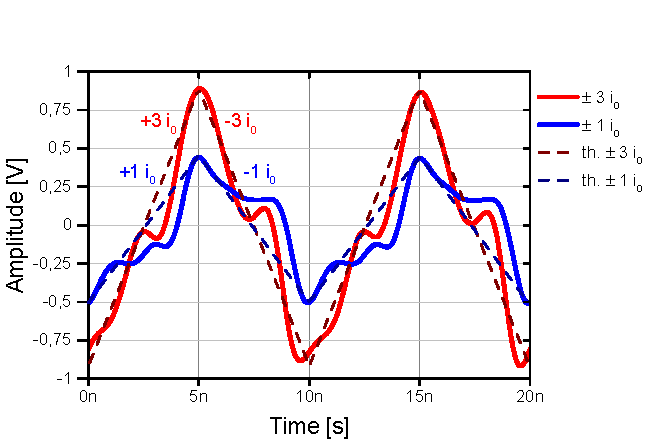
\includegraphics{100M_Cload_regression.pdf}
	\caption{time domain measurement with capacitive load at fs = 100MHz}
	\label{fig:measCload100M}
\end{figure}

The red signal represents a synthesized triangular waveform with a slope corresponding to $3 i_0$, while the brown dashed signal provides the theoretical signal.\\
The blue signal represents a synthesized triangular waveform with a slope corresponding to $1 i_0$, while the dashed darker blue signal provides the theoretical one.\\
The same notation is valid for the synthesized signal in figure \ref{fig:measCload150M}.
Here the signal frequency is \SI{150}{\mega \hertz} which is the upper bound for this measurement setup.
The signal integrity is much worse going beyond this frequency.

\begin{figure}[htb!]
	\centering
  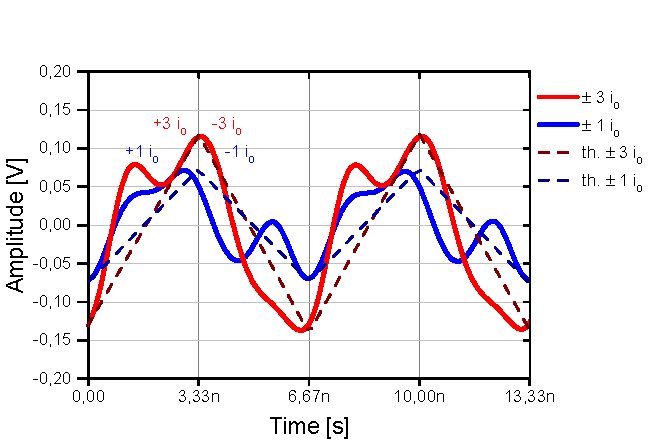
\includegraphics{150M_Cload_regression.pdf}
	\caption{time domain measurement with capacitive load at fs = 150MHz}
	\label{fig:measCload150M}
\end{figure}

%Although the difference between the relative slope of $3 i_0$ and $1 i_0$ is much less the signal can 
The difference between the slopes is getting smaller while the signal quality is decreasing.


\section{Discussion of measurement results}
In a first step it was shown that the designed circuit converts a digital signal to an analog one.
The frequency limit for this measurement setup consisting of this designed circuit is at roughly \SI{150}{\mega \hertz}.
Heat is critical. 
Aside from some parasitic effects the proof of the concept was successful.

%\textit{is it possible to measure the heat spreading on the substrate?}
%Is the measurement result expected due to the simulation? Can the demonstrator be simulated although no model for this chips exists? The real simulation are not done due to the fact that no losses respected.

% Compare and evaulate the simulation to the measurement
